\section{手写数字及写字人识别实验过程及其结果}

\subsection{手写数字识别实验}

\subsubsection{样本简介}
本论文的手写数字识别实验当中所用的样本分为两类,一类是训练样本集,另一类是测试样本集。\\
\hspace*{\parindent}实验当中的训练样本集采用的是手写数字MNIST数据库。这个数据库当中包含训练集样本60000个样例和测试集样本10000个样例。
MNIST数据库当中的数字样本已经全部大小归一化灰度化并且集中到同一个固定大小的图像当中。
该数据库包括MST的SD-1和SD-3数据库,当中包含一系列的二级制的手写数字图像。
其中SD-1的收集者来源是某高中的在校学生,而SD-3是由人口调查局员工收集的。
则我们的训练样本集也就是MNIST当中的训练样本集有30000个样本来自SD-3,而另外30000个样本来自SD-1。这60000个训练样本分别来自约250个采集者。

\subsubsection{Writer Depend类数字识别实验}
......

\paragraph{ABCvsA数字识别实验}
\hspace*{\parindent}实验内容:以A写字人、B写字人和C写字人,合计3000个数字0到9的数字图像数据为训练样本集。
A写字人的1000个数字0到9的数字图像数据为测试样本集。学习率为1,单次训练样本数为10个,共训练40次。
若识别所得数字与给定的标签匹配,则视为正确;不匹配则视为错误。
\begin{table}[!htbp]
    \centering
    \caption{ABCvsA数字识别实验结果}
    \begin{tabular}[\textwidth]{c|c|c|c}
        \hline
        训练样本 & ABC & 样本个数 & 3000 \\
        \hline
        测试样本 & A & 样本个数 & 1000 \\
        \hline
        训练样本 & $\backslash$ & 单次训练样本数 & 10 \\
        \hline
        学习率 & 1 & 正确率 & 99.50\% \\
        \hline
    \end{tabular}
\end{table}

\paragraph{ABCvsABC数字识别实验}
\hspace*{\parindent}实验内容:以A写字人、B写字人和C写字人,合计3000个数字0到9的数字图像数据为总样本集。
在总样本集当中随机抽取2400个为训练样本集,余下的600个为测试样本集。
学习率为1,单次训练样本数为10个,共训练40次。若识别所得数字与给定的标签匹配,则视为正确;不匹配则视为错误。
\begin{table}[!htbp]
    \centering
    \caption{ABCvsABC数字识别实验结果}
    \begin{tabular}[\textwidth]{c|c|c|c}
        \hline
        训练样本 & ABC & 样本个数 & 2400 \\
        \hline
        测试样本 & ABC & 样本个数 & 600 \\
        \hline
        训练样本 & 40 & 单次训练样本数 & 10 \\
        \hline
        学习率 & 1 & 正确率 & 92.00\% \\
        \hline
    \end{tabular}
\end{table}

\subsubsection{Writer Depend类数字识别实验结果分析}
下面我们选取Writer Depend类数字识别实验当中的两个典型的例子ABCvsA数字识别实验以及MNIST\& ABCvsA数字识别实验的结果做详细分析。
我们从ABCvsA数字识别实验中的训练样本集和测试样本集的手写数字图像样本集当中分别随机抽取一幅图像如图4-1所示。\\
\hspace*{\parindent}下面我们对上述的训练集和测试集进行40次学习率为2,单次训练样本为10的迭代,得到错误率为0.50\%,而其中每次训练时的误差值组成的历史误差值画图分析如下:\\
\hspace*{\parindent}......

\begin{figure}[!htbp]
    \centering
    \subfigure[实验训练集]{
      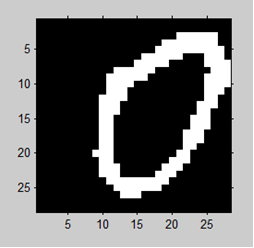
\includegraphics[width=0.45\textwidth]{figs/train.png}
      \label{fig:train}
    }
    \subfigure[实验测试集]{
      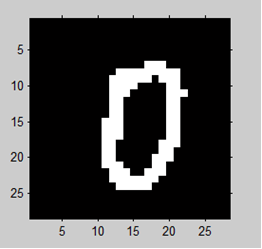
\includegraphics[width=0.45\textwidth]{figs/test.png}
      \label{fig:test}
    }
    \caption{ABCvsA数字识别实验集}
    \label{fig:both_images}
\end{figure}

\subsubsection{Writer Independ类数字识别实验}
实验内容:以MNIST数据库为训练样本集,共计60000个训练样本。以A写字人合计1000个数字0到9的数字图像数据为测试样本集写字人识别实验\\
\hspace*{\parindent}......

\subsubsection{样本简介}
......

\subsubsection{两位写字人识别实验}
\paragraph{单个数字的写字人识别实验}
\hspace*{\parindent}实验内容:以A写字人,合计800个数字5的数字图像数据加上B写字人,合计800个数字5的数字图像数据,
共计1600个样本为总样本集。随机选取其中的1200个样本为训练样本集,其余的400个样本为测试样本集。学习率为2,
单次训练样本数为10个,共训练30次。若识别所得写字人与给定的标签匹配,则视为正确;不匹配则视为错误。
\begin{table}[!htbp]
    \centering
    \caption{单个数字写字人识别实验结果}
    \begin{tabular}[\textwidth]{c|c|c|c}
        \hline
        训练样本 & A5\&B5 & 样本个数 & 1200 \\
        \hline
        测试样本 & A5\&B5 & 样本个数 & 400 \\
        \hline
        训练样本 & 30 & 单次训练样本数 & 10 \\
        \hline
        学习率 & 2 & 正确率 & 99.75\% \\
        \hline
    \end{tabular}
\end{table}

\paragraph{单个数字的写字人识别实验结果分析}
\hspace*{\parindent}......

\subsection{本章小结}
......

\newpage
